\section{Introduktion till mixnät}
\begin{frame}
\frametitle{Innehåll}
\tableofcontents[currentsection]
\end{frame}

\begin{frame}{Mixnät - En digital tombola}

\begin{columns}
    \begin{column}{0.4\textwidth}
        \begin{itemize}
			\item Indata:
			\begin{itemize}
				\item[-] Krypterade röster
			\end{itemize}
			\item[]
			\item Körning:
			\begin{itemize}
				\item[-] Blandas hemligt
			\end{itemize}
			\item[]
			\item Utdata:
			\begin{itemize}
				\item[-] Dekrypterade röster
			\end{itemize}
		\end{itemize}
    \end{column}
	\begin{column}{0.6\textwidth}
    	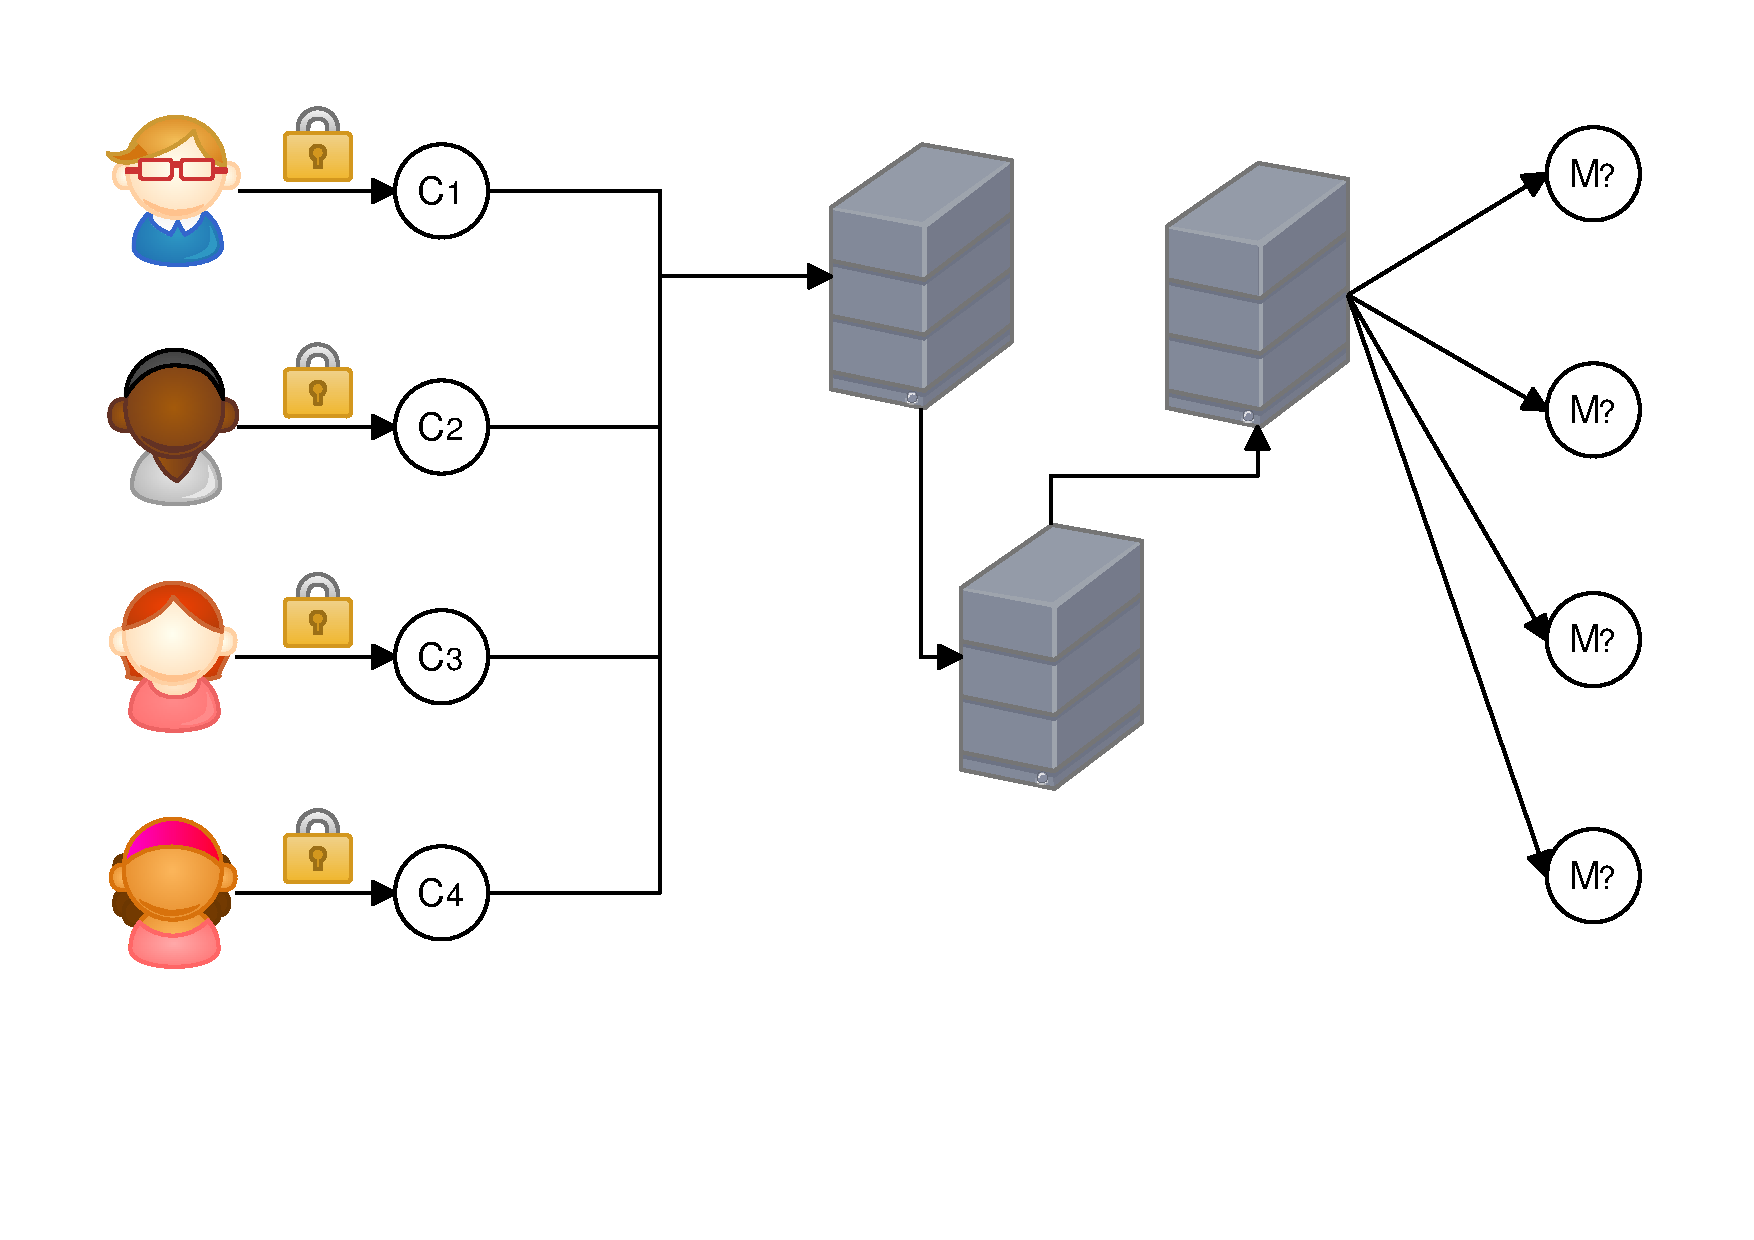
\includegraphics[height=0.7\textwidth]{images/mix1.pdf}
	\end{column}
\end{columns}

\end{frame}